%Assignment 2 
%Vikas Kurapati
%130010058
\documentclass[11pt, a4paper]{article}
\usepackage[affil-it]{authblk} 
\usepackage{etoolbox}
\usepackage{lmodern}
\usepackage{titlesec}
\usepackage{float}

\makeatletter
\patchcmd{\@maketitle}{\LARGE \@title}{\fontsize{20}{19.2}\selectfont\@title}{}{}
\makeatother

\renewcommand\Authfont{\fontsize{16}{14.4}\selectfont}
\renewcommand\Affilfont{\fontsize{12}{10.8}\itshape}

\title{\textbf{Assignment 3}} 
\author{Vikas Kurapati - 130010058}
\usepackage{graphicx}
\begin{document}
\maketitle
\newpage
\section{Question1:}
The following plots show the results of the simulation of a charged particle motion under the influence of a constant magnetic field and no electric field.
\subsection{Paths using Different Schemes}
Refer code for the values used for the simulation.
\begin{figure}[H]
 \centering
 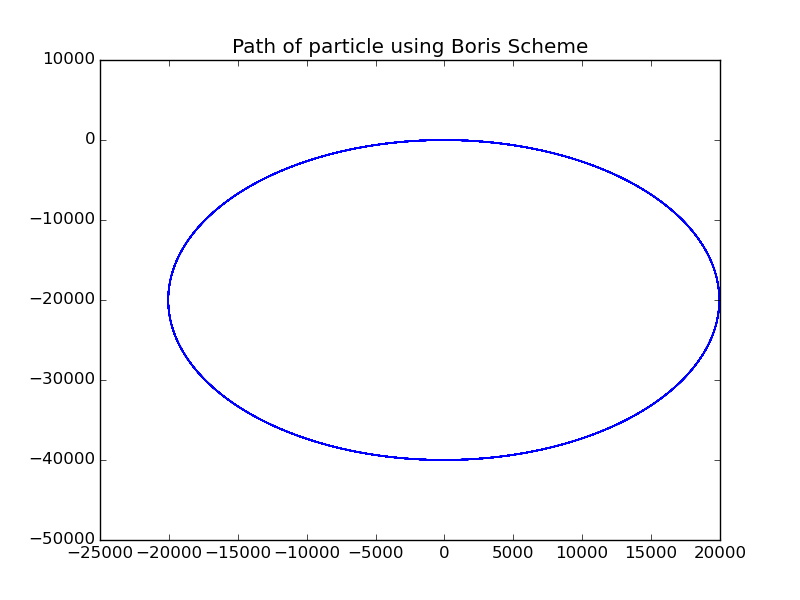
\includegraphics[width = \textwidth]{q1_path_boris.png}
\end{figure}
\begin{figure}[H]
 \centering
 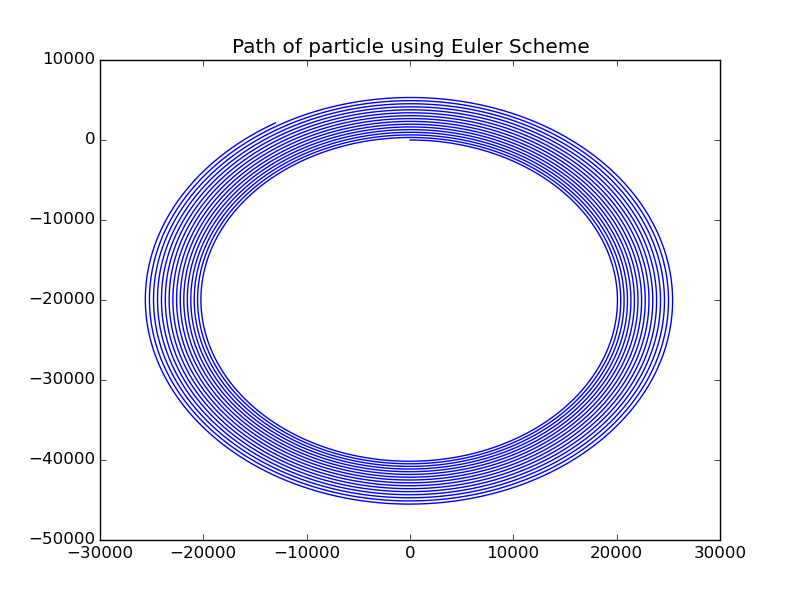
\includegraphics[width = \textwidth]{q1_path_euler.png}
\end{figure}
\begin{figure}[H]
 \centering
 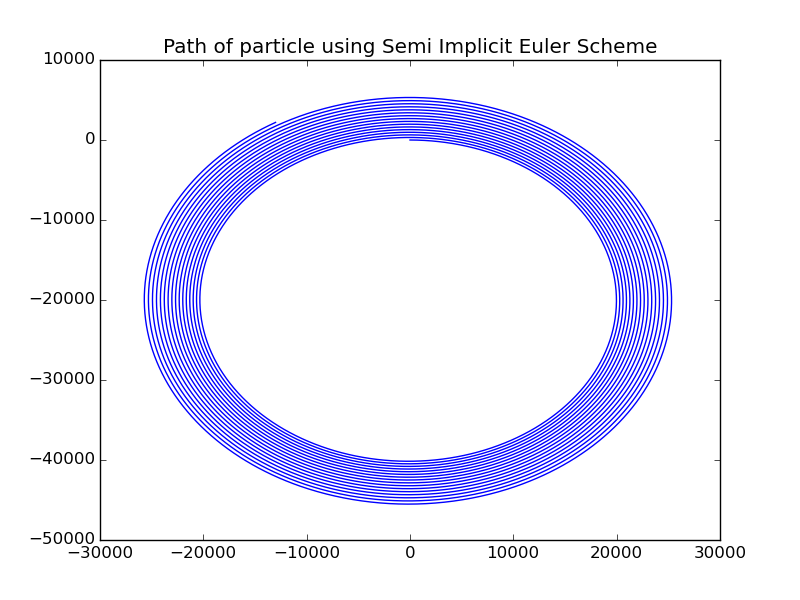
\includegraphics[width = \textwidth]{q1_path_euler2.png}
\end{figure}
\begin{figure}[H]
 \centering
 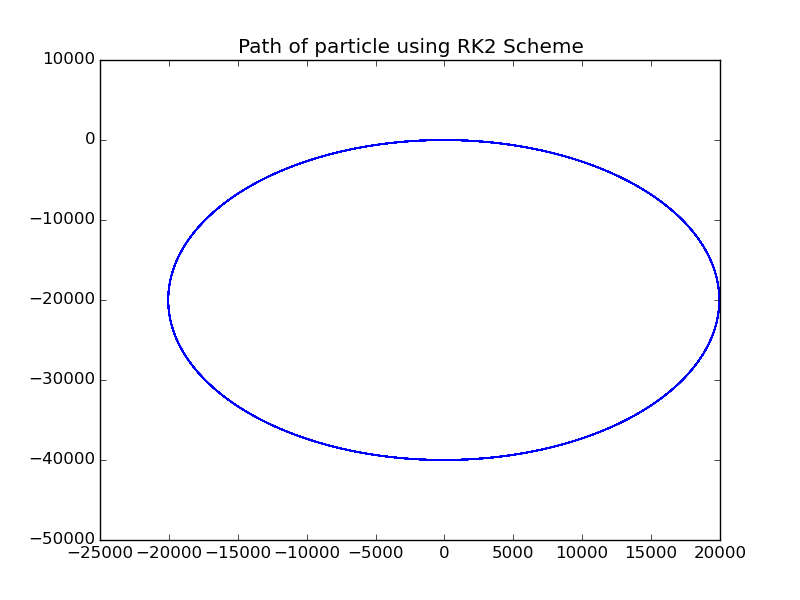
\includegraphics[width = \textwidth]{q1_path_RK2.png}
\end{figure}

\subsection{Energy Development with time using Different Schemes}
\begin{figure}[H]
 \centering
 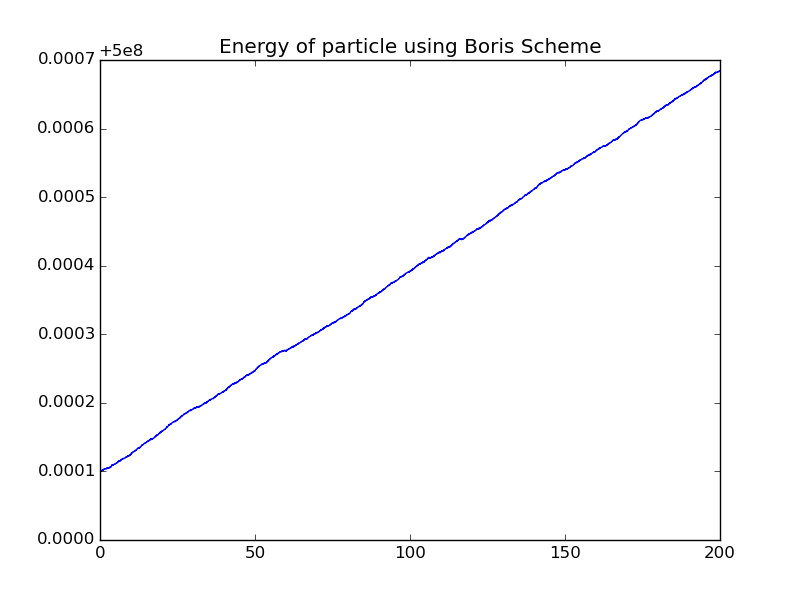
\includegraphics[width = \textwidth]{q1_energy_boris.png}
\end{figure}
\begin{figure}[H]
 \centering
 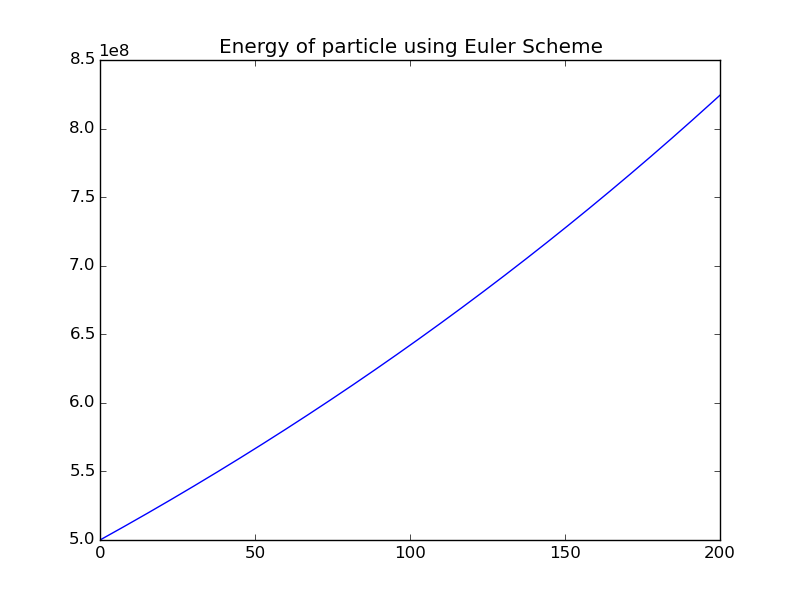
\includegraphics[width = \textwidth]{q1_energy_euler.png}
\end{figure}
\begin{figure}[H]
 \centering
 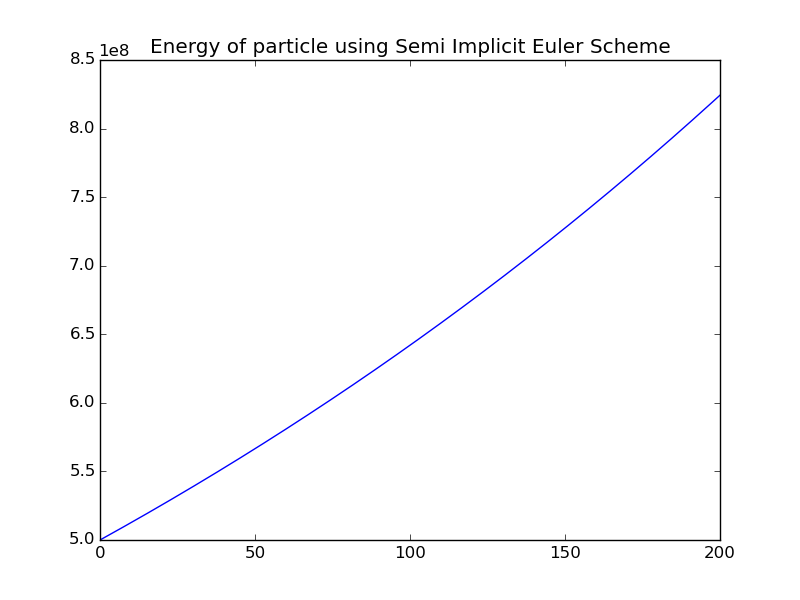
\includegraphics[width = \textwidth]{q1_energy_euler2.png}
\end{figure}
\begin{figure}[H]
 \centering
 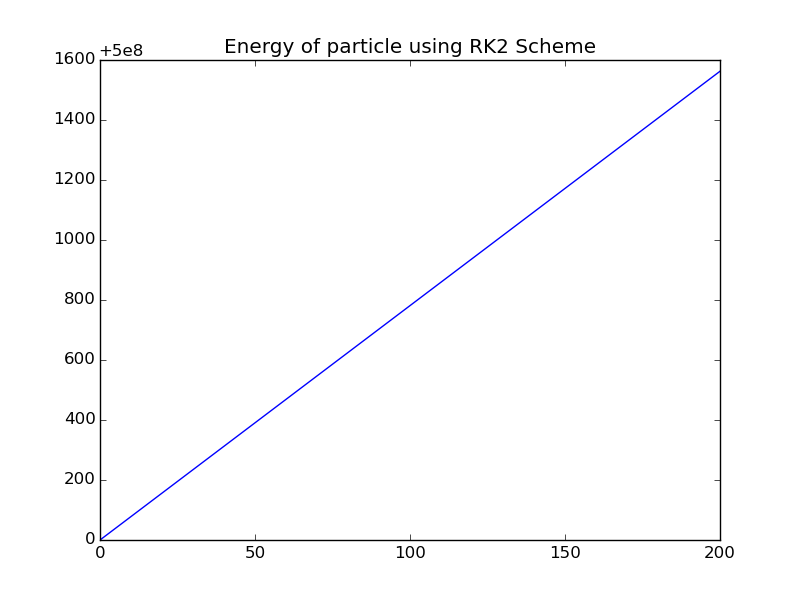
\includegraphics[width = \textwidth]{q1_energy_RK2.png}
\end{figure}

\subsection{Dissipation of energy with time using Different Schemes}
\begin{figure}[H]
 \centering
 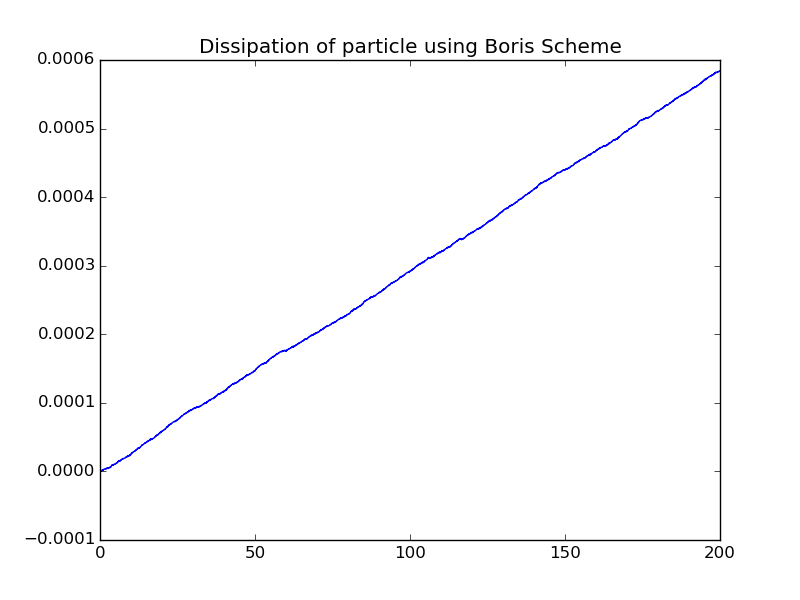
\includegraphics[width = \textwidth]{q1_dissipation_boris.png}
\end{figure}
\begin{figure}[H]
 \centering
 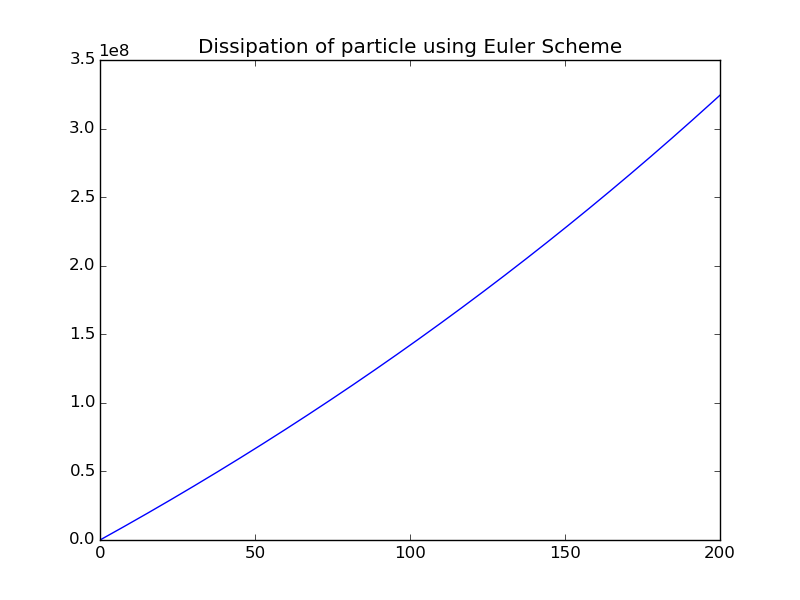
\includegraphics[width = \textwidth]{q1_dissipation_euler.png}
\end{figure}
\begin{figure}[H]
 \centering
 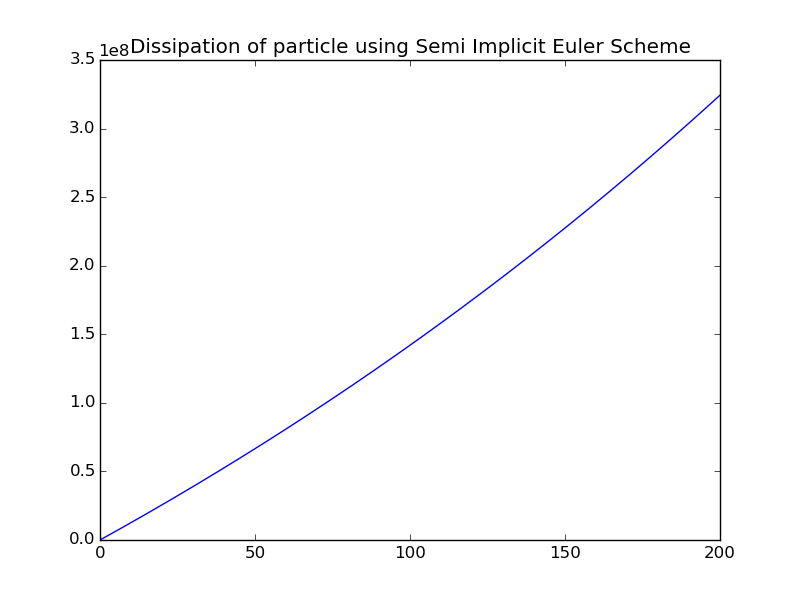
\includegraphics[width = \textwidth]{q1_dissipation_euler2.png}
\end{figure}
\begin{figure}[H]
 \centering
 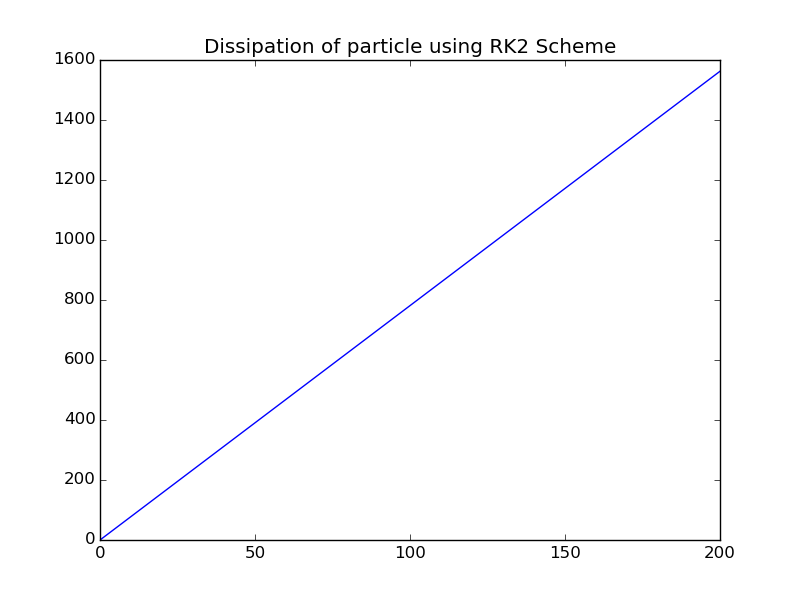
\includegraphics[width = \textwidth]{q1_dissipation_RK2.png}
\end{figure}

\subsection{Error in Particle Position with time using Different Schemes}
\begin{figure}[H]
 \centering
 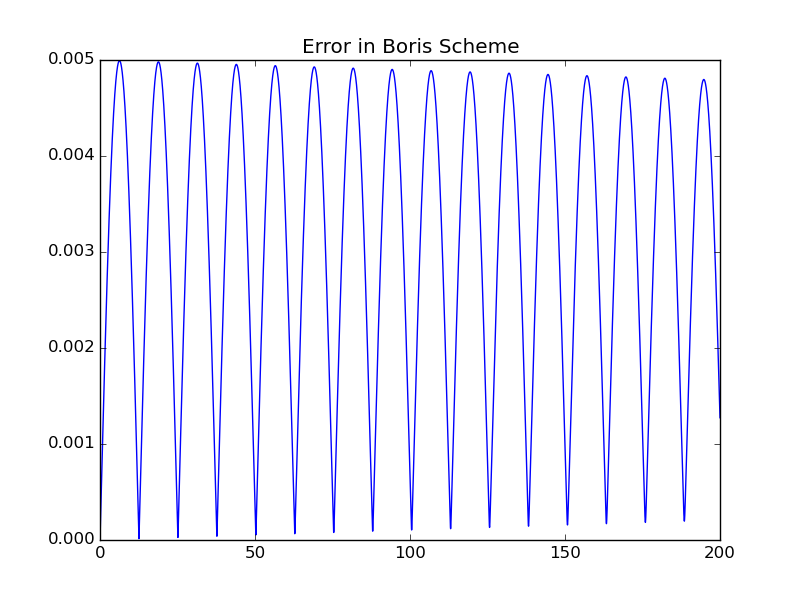
\includegraphics[width = \textwidth]{q1_error_boris.png}
\end{figure}
\begin{figure}[H]
 \centering
 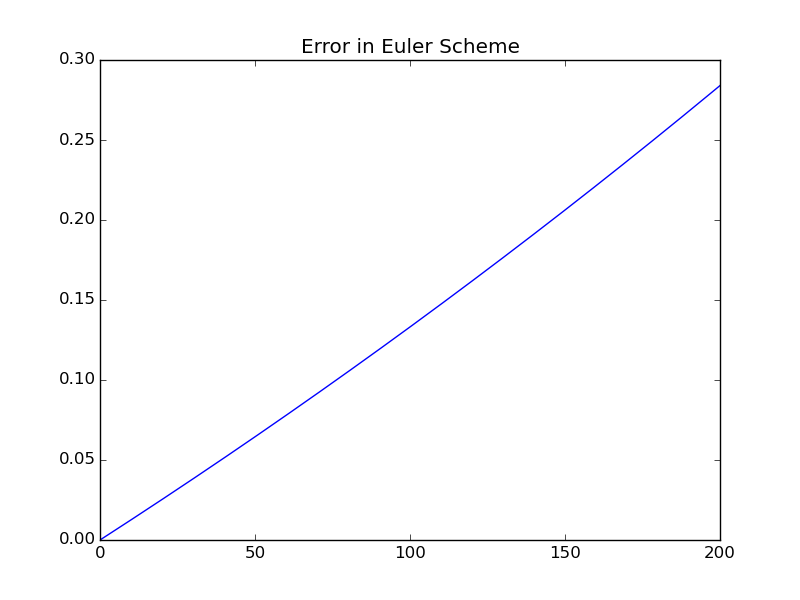
\includegraphics[width = \textwidth]{q1_error_euler.png}
\end{figure}
\begin{figure}[H]
 \centering
 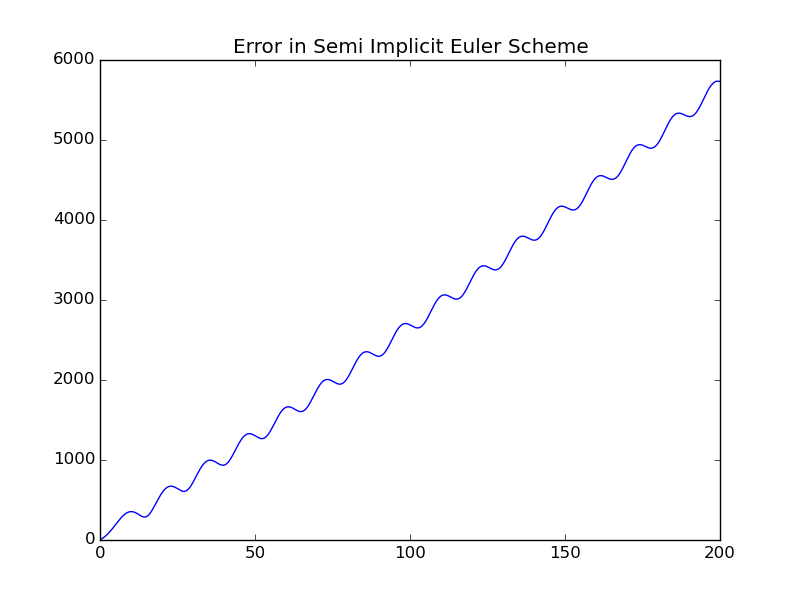
\includegraphics[width = \textwidth]{q1_error_euler2.png}
\end{figure}
\begin{figure}[H]
 \centering
 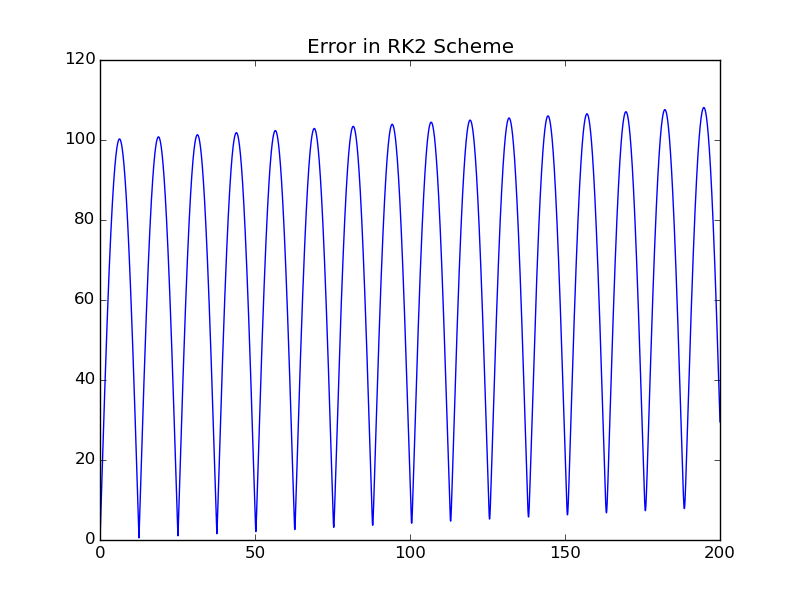
\includegraphics[width = \textwidth]{q1_error_RK2.png}
\end{figure}

\section{Question 2}
Error in different schemes varying with time step size for the constant magnetic field simulation.
\begin{figure}[H]
 \centering
 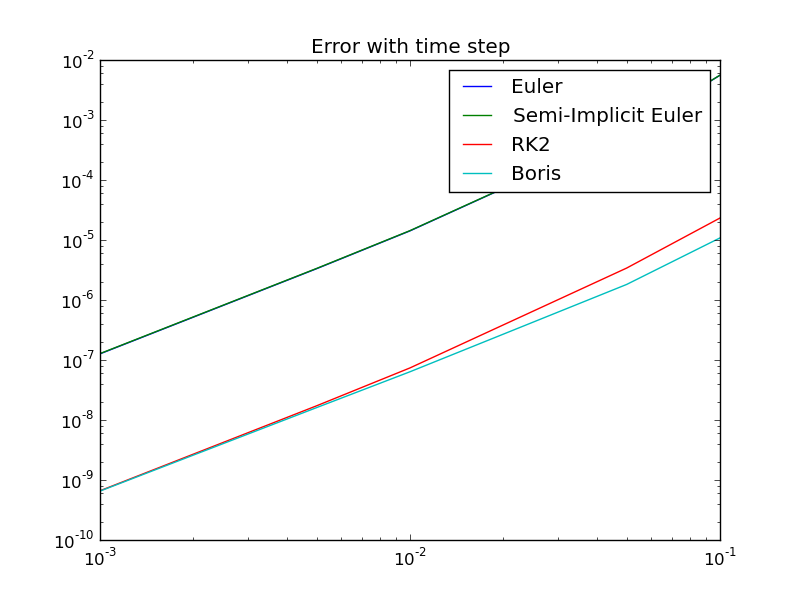
\includegraphics[width = \textwidth]{q2_Error.png}
\end{figure}

It can be clearly seen that the slope of RK2 is greater than Euler showing the orders of the schemes to be 2 and 1 respectively as the plot is a log log plot.

\section{Question 3}
The following plots show the results of motion of a charged particle under the influence of a constant electric field and magnetic field.
\subsection{Paths using Different Schemes}
\begin{figure}[H]
 \centering
 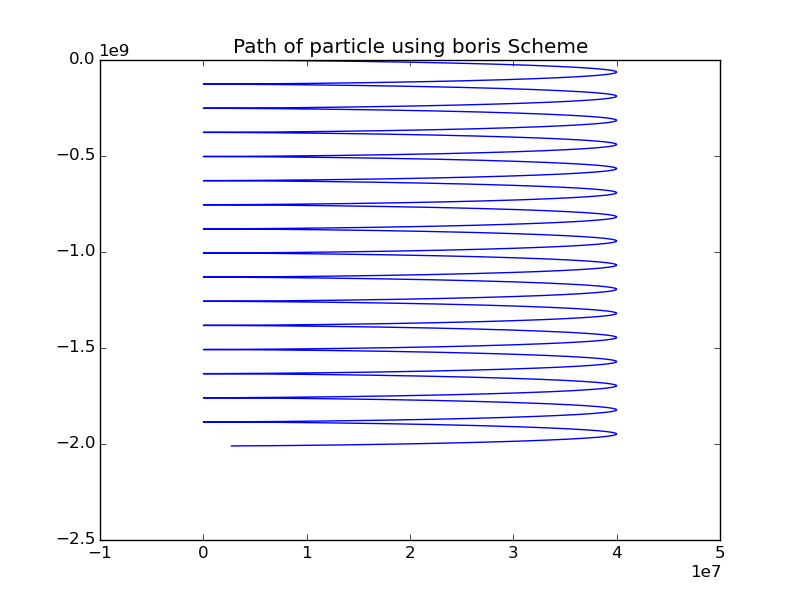
\includegraphics[width = \textwidth]{q3_boris.png}
\end{figure}
\begin{figure}[H]
 \centering
 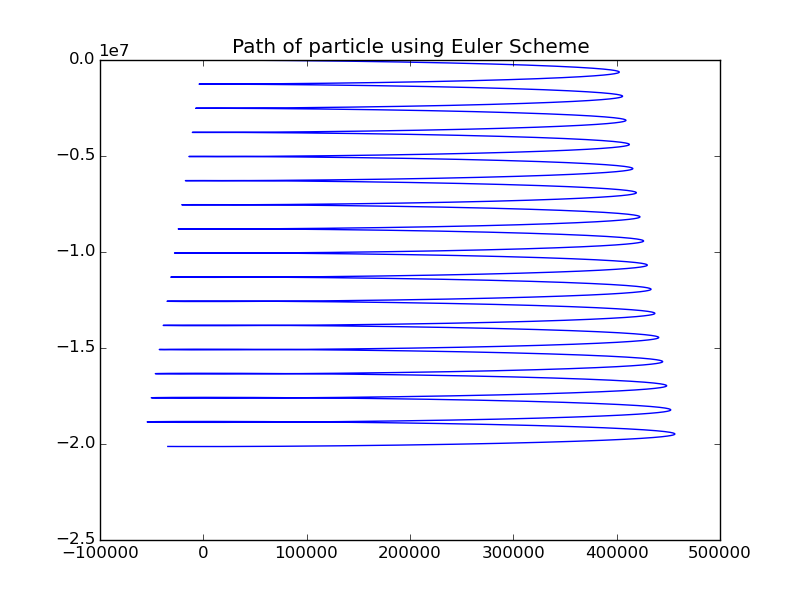
\includegraphics[width = \textwidth]{q3_euler.png}
\end{figure}
\begin{figure}[H]
 \centering
 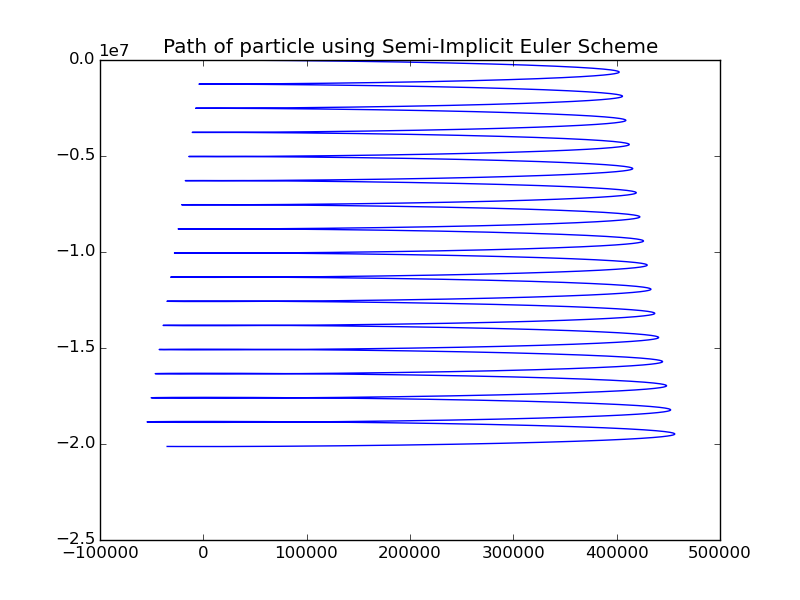
\includegraphics[width = \textwidth]{q3_euler2.png}
\end{figure}
\begin{figure}[H]
 \centering
 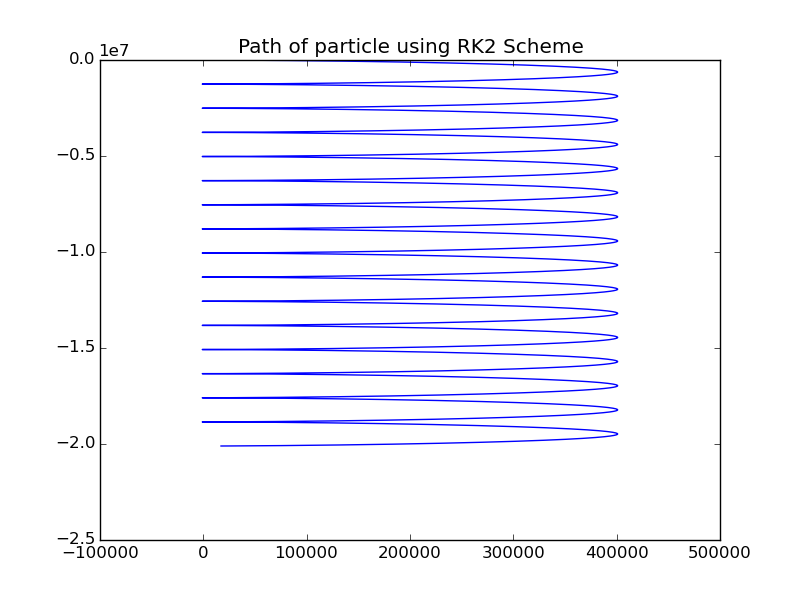
\includegraphics[width = \textwidth]{q3_RK2.png}
\end{figure}

\subsection{Error in Particle Position with time using Different Schemes}
\begin{figure}[H]
 \centering
 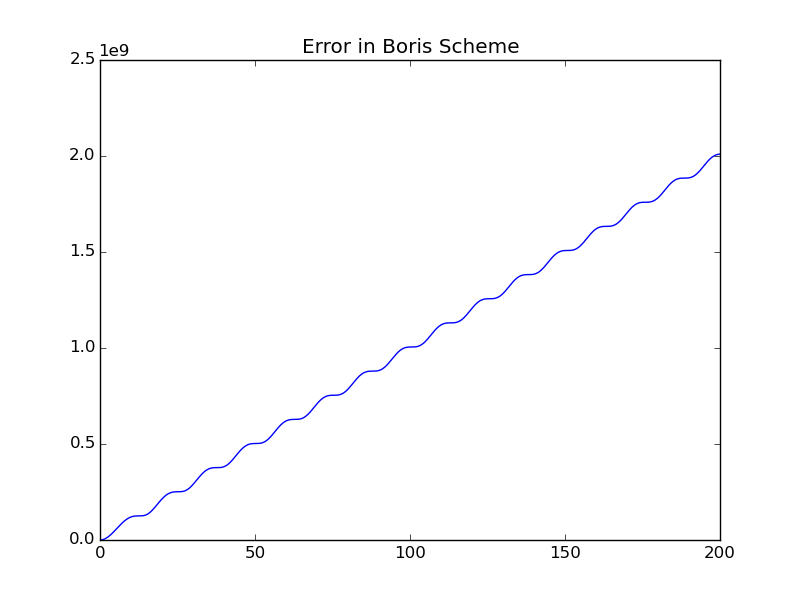
\includegraphics[width = \textwidth]{q3_error_boris.png}
\end{figure}
\begin{figure}[H]
 \centering
 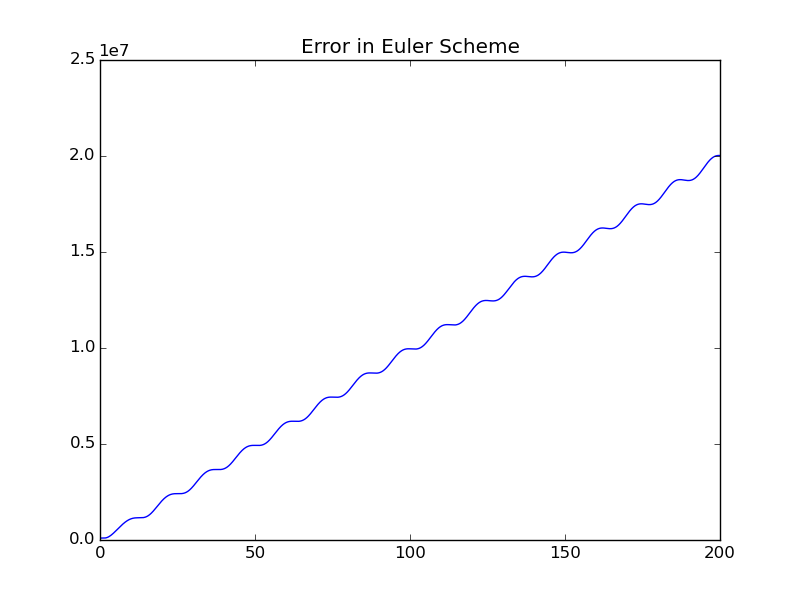
\includegraphics[width = \textwidth]{q3_error_euler.png}
\end{figure}
\begin{figure}[H]
 \centering
 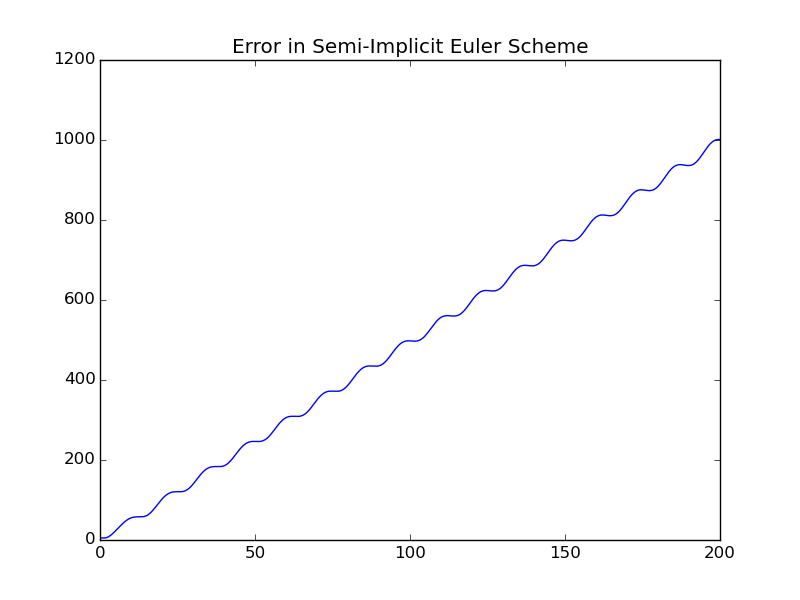
\includegraphics[width = \textwidth]{q3_error_euler2.png}
\end{figure}
\begin{figure}[H]
 \centering
 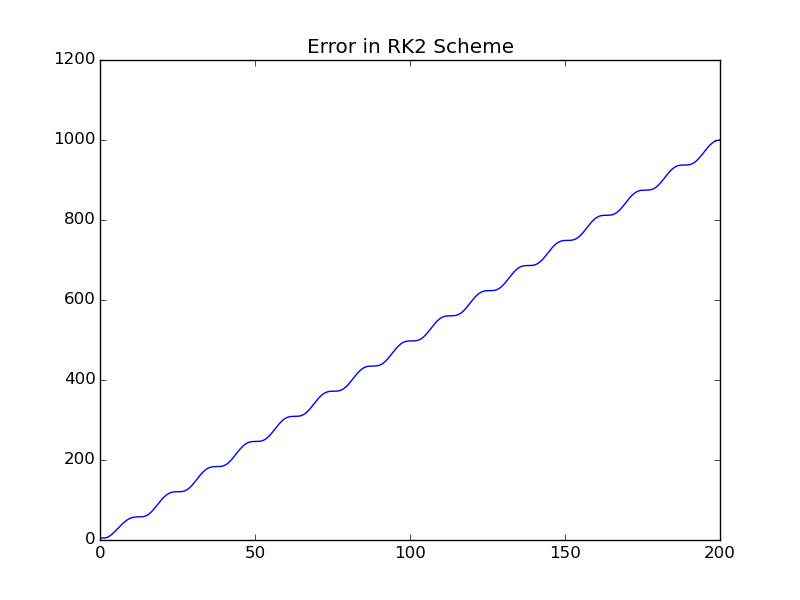
\includegraphics[width = \textwidth]{q3_error_RK2.png}
\end{figure}

\section{Question 4}
The following plots show the results of motion of a charged particle under the influence of a zero electric field and constant gradient magnetic field whose z-component's gradient is constant along x-axis.
\subsection{Paths using Different Schemes}
\begin{figure}[H]
 \centering
 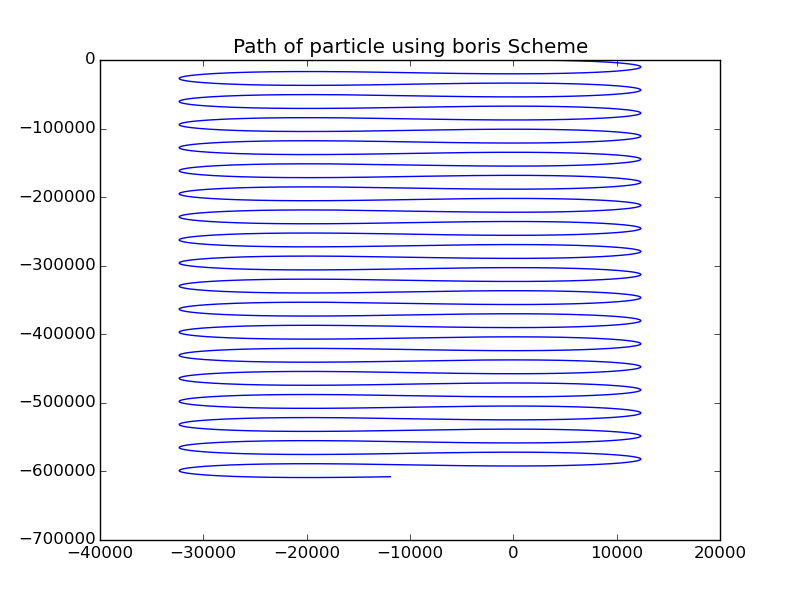
\includegraphics[width = \textwidth]{q4_boris.png}
\end{figure}
\begin{figure}[H]
 \centering
 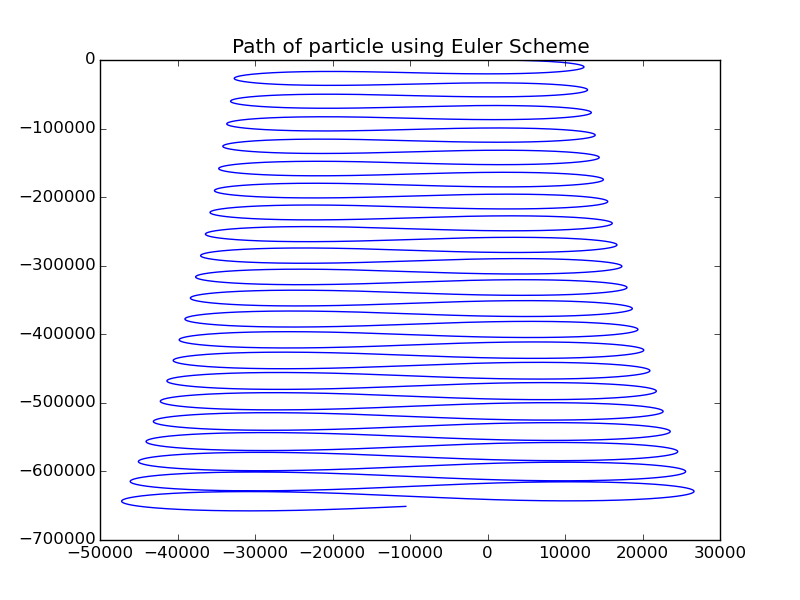
\includegraphics[width = \textwidth]{q4_euler.png}
\end{figure}
\begin{figure}[H]
 \centering
 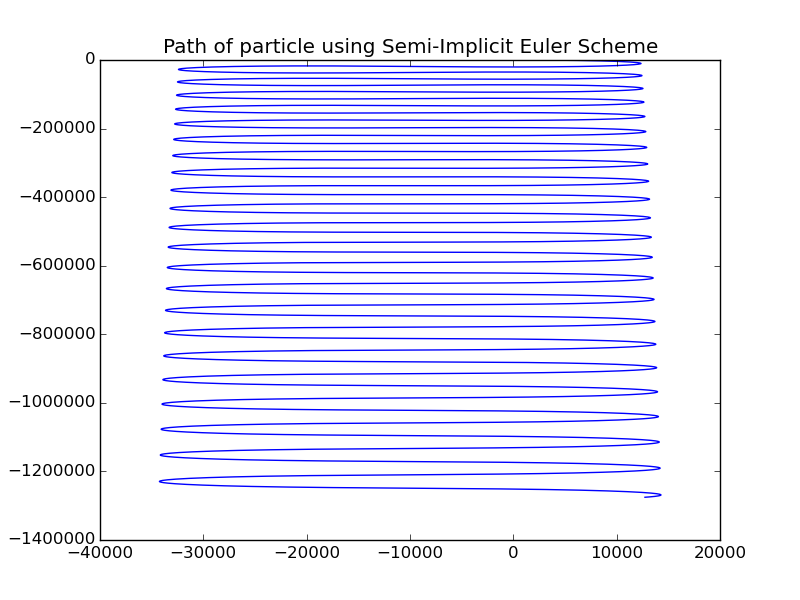
\includegraphics[width = \textwidth]{q4_euler2.png}
\end{figure}
\begin{figure}[H]
 \centering
 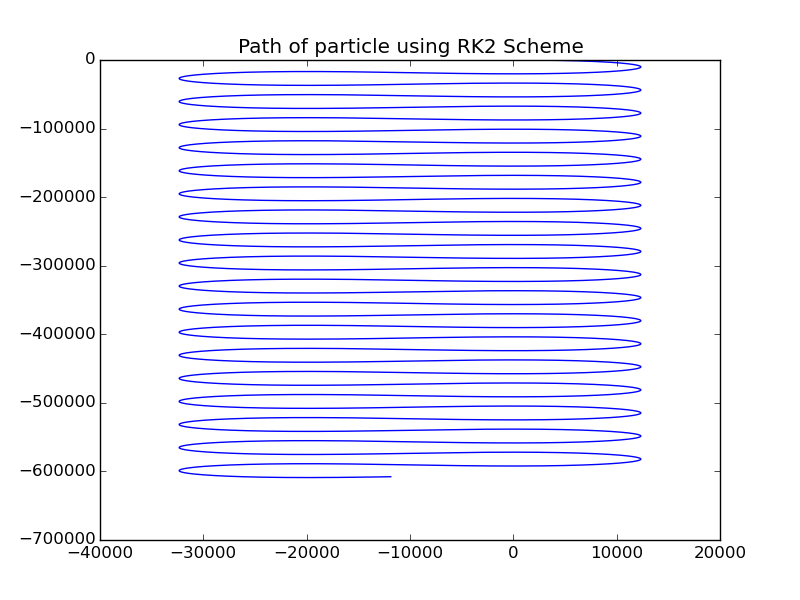
\includegraphics[width = \textwidth]{q4_RK2.png}
\end{figure}

\subsection{Error in Particle Position with time using Different Schemes}
\begin{figure}[H]
 \centering
 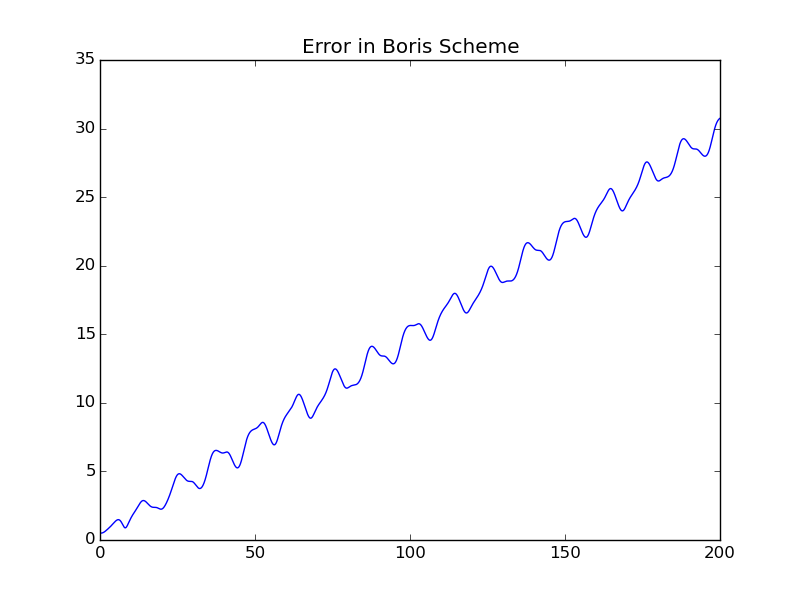
\includegraphics[width = \textwidth]{q4_error_boris.png}
\end{figure}
\begin{figure}[H]
 \centering
 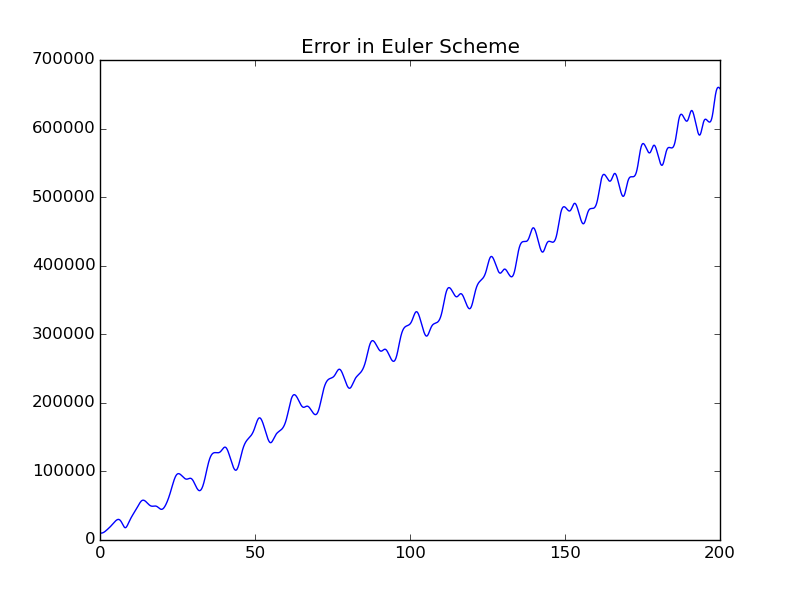
\includegraphics[width = \textwidth]{q4_error_Euler.png}
\end{figure}
\begin{figure}[H]
 \centering
 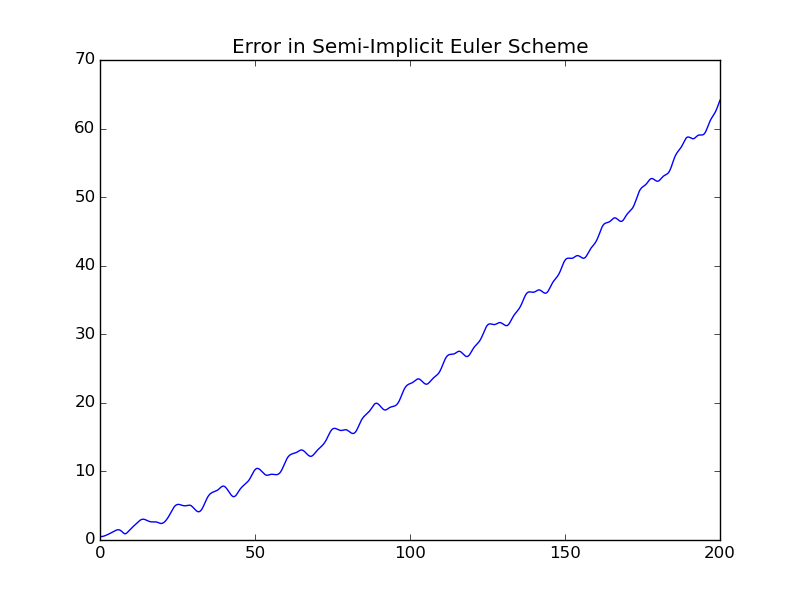
\includegraphics[width = \textwidth]{q4_error_euler2.png}
\end{figure}
\begin{figure}[H]
 \centering
 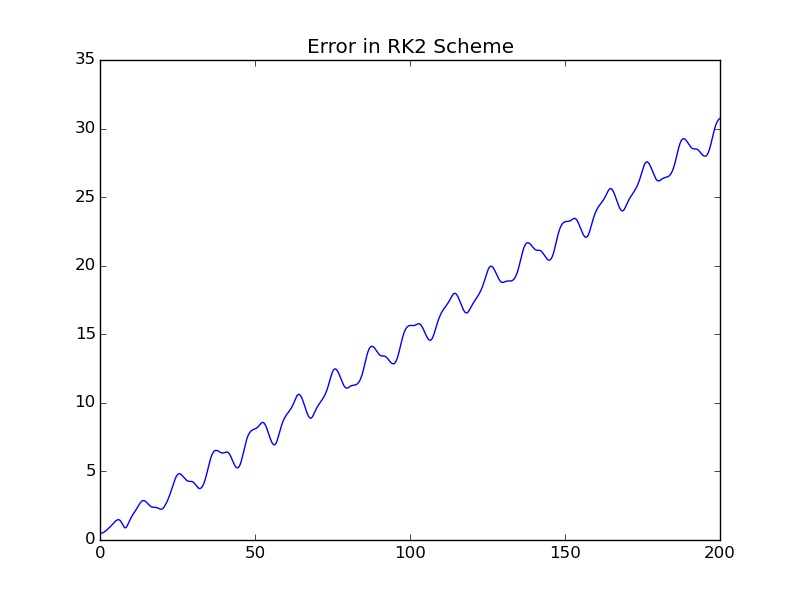
\includegraphics[width = \textwidth]{q4_error_RK2.png}
\end{figure}

\end{document}